\documentclass[11pt]{article}
\usepackage{amsmath,amssymb,amsthm,graphicx,hyperref,booktabs,longtable,enumitem}
\usepackage[margin=1in]{geometry}
\usepackage{natbib}
\usepackage{xurl}
\usepackage{seqsplit}
\usepackage{array}
\usepackage{ragged2e}

\graphicspath{{figures/}}
% Breakable repo paths and Lean identifiers.
% Declared robust so they survive moving arguments (\paragraph writes its
% argument to the .toc, where the fragile \path/\url machinery otherwise
% expanded and raised "\url used in a moving argument".)
\DeclareRobustCommand{\repopath}[1]{\path{#1}}
\DeclareRobustCommand{\leanthm}[1]{\path{#1}}
\DeclareRobustCommand{\leanfile}[1]{\path{#1}}
% Safe in \paragraph / PDF bookmarks (TOC-safe headings)
\DeclareRobustCommand{\leanhdr}[1]{\texorpdfstring{\leanthm{#1}}{#1}}
% Allow modest line-stretch, as in the main manuscript, so long identifiers in
% justified prose do not overflow the measure.
\emergencystretch=2em

\newtheorem{theorem}{Theorem}
\newtheorem{lemma}{Lemma}
\newtheorem{corollary}{Corollary}
\newtheorem{definition}{Definition}
\newtheorem{remark}{Remark}

\title{Supplementary Material\\
\large ChiralFold: systematic detection of D-amino acid stereochemistry errors in the Protein Data Bank}
\author{Tommaso R. Marena}
\date{}

\begin{document}
\maketitle

\tableofcontents
\vspace{1em}

\section{Supplementary Methods}

\subsection{Ramachandran benchmark protocol}
Era-representative stratified sampling across X-ray ultra ($\leq$1.20~\AA), high, medium, low, NMR, and cryo-EM bins (seed 20260612). mmCIF$\to$PDB conversion uses chain-ID remapping (A--Z, 0--9). Structures with $>$36 distinct chains skipped. Script: \repopath{benchmarks/expand_ramachandran_benchmark.py}.

\subsection{Experimental validation protocol}
Automated cross-check of all 16 error structures: \repopath{benchmarks/experimental_structure_validation.py} queries RCSB entry metadata (method, resolution) and wwPDB CCD InChI stereochemistry; results in \repopath{results/experimental_validation_report.json}. Reproduce in Colab: \repopath{demos/D_Residue_Experimental_Validation.ipynb}. PDB 5M2K exclusion: \repopath{results/5m2k_benchmark_exclusion.json}.

\subsection{Mirror-image, AF3 correction, and enumeration}
L$\leftrightarrow$D reflection: $(x,y,z)\to(-x,y,z)$. Because reflection is an isometry, all pairwise distances (and therefore MolProbity-style clashscore) are unchanged before vs.\ after mirroring (\repopath{tests/test_clash_preservation.py}). AF3 correction reflects only the violating C$\alpha$ (and HA if present) across the N--C--C$\beta$ plane, preserving CA--N, CA--C, and CA--C$\beta$ bond lengths exactly and driving residual chirality violations to 0\%. Diastereomer enumeration scores $2^k$ L/D patterns. Interface scoring uses BSA, H-bonds, and salt bridges.

\subsection{Clashscore implementation}
ChiralFold clashscore counts non-bonded atom pairs with van der Waals overlap $\geq$0.4~\AA\ (KD-tree neighbour search), reported per 1000 heavy atoms. Radii follow Bondi for heavy atoms and Probe-like $1.17$~\AA\ for hydrogen. Implementation details:
\begin{itemize}[leftmargin=*]
  \item \textbf{First MODEL only} for multi-model (NMR) files.
  \item \textbf{Strip deposited hydrogens}, then place (i)~backbone amide HN (MolProbity Reduce-style; proline skipped; same-chain peptide-continuous neighbours only, including insertion codes) and (ii)~C$\alpha$ hydrogens---HA for residues with C$\beta$, and HA2/HA3 for glycine.
  \item \textbf{Exclude covalent 1--2 / 1--3 / 1--4} contacts using standard amino-acid topology (not a brittle distance cutoff), so pairs such as LEU CA--CG are never scored as clashes; for pairs involving a model-built hydrogen, also exclude same-residue 1--5 and peptide 1--5 contacts such as O($i$)--HA($i{+}1$).
  \item \textbf{Exclude} disulfide SG--SG bridges.
  \item \textbf{H-bond geometry gate:} a polar H$\cdots$acceptor contact suppresses a clash only if H$\cdots$Acc $\leq$2.5~\AA\ and the donor--H--Acc angle is $\geq$120$^\circ$; heavy N$\cdots$O pairs only in the 2.5--3.5~\AA\ window. Carbon-bound HA/HA2/HA3 are never treated as H-bond donors.
\end{itemize}
Clashscore feeds the composite 0--100 quality score (15 of 100 points) in the CLI/web UI. It is \emph{not} an input to the PDB-wide D-residue survey (signed volume only; independent numpy verifier) nor to the primary Ramachandran calibration ($n=362$). A secondary 31-structure MolProbity head-to-head panel (\repopath{results/molprobity_comparison.json}) was regenerated after these rules: mean ChiralFold clashscore~$27.4$ (wwPDB panel mean~$18.0$; median CF~$15.3$). An earlier distance-gated implementation that scored covalent 1--3 contacts and deposited hydrogens inflated the same panel mean to $\sim$265 and is superseded. Tests: \repopath{tests/test_clash_exclusions.py}, \repopath{tests/test_clash_preservation.py}.

\subsection{Structure input formats and remote fetch}
CLI and Gradio (local / Hugging Face Space) accept:
\begin{itemize}[leftmargin=*]
  \item Local \textbf{PDB} (\texttt{.pdb}/\texttt{.ent}), \textbf{mmCIF} (\texttt{.cif}/\texttt{.mmcif}; in-core \texttt{\_atom\_site}$\to$PDB conversion with chain-ID remapping; no gemmi required in the core package), and \textbf{FASTA} with a UniProt accession in the header (resolved via AlphaFold~DB when online).
  \item Optional network fetch: RCSB by 4-character PDB ID; AlphaFold~DB by UniProt accession or \texttt{AF-\ldots-Fn} tag (\repopath{chiralfold/fetch.py}).
\end{itemize}
Commands: \texttt{chiralfold fetch}, \texttt{chiralfold audit --id}, \texttt{chiralfold correct-af3 --id}. Fetch is download-only---ChiralFold does not run AF2/Boltz/AF3 inference. The Space prefers bundled CSS and exposes an in-app Light/Dark theme toggle (\texttt{?\_\_theme=light|dark}).

\subsection{Unusual cases: macrocycles, non-standard ligands, and density}
The signed-volume C$\alpha$ classifier does not require standard protein geometry. Representative edge cases (\repopath{demos/Demo_Unusual_Cases_Clash_Safety.ipynb}):
\begin{itemize}[leftmargin=*]
  \item \textbf{Cyclic / strained peptides:} PDB 1XT7 (daptomycin) and 2RMI (astressin).
  \item \textbf{Non-standard CCD ligands:} PDB 1OF6 (eight DTY$\leftarrow$L-Tyr); 1BG0/1P52 (DAR$\leftarrow$L-Arg).
  \item \textbf{High-resolution density:} PDB 1HHZ (0.99~\AA) DAL error.
  \item \textbf{Non-protein Rama exclusion:} PDB 5M2K (vancomycin glycopeptide).
\end{itemize}

\subsection{Five-minute offline reproduction}
\repopath{python benchmarks/reproduce_d_residue_errors.py} (numpy only; Colab: \repopath{demos/Reproduce_PDB_D_Residue_Errors_5min.ipynb}).

\subsection{mmCIF known-error re-verification and universe survey}
The primary survey used legacy PDB files. We subsequently (i)~re-parsed all 16 known-error structures from native RCSB mmCIF and (ii)~enumerated the live mmCIF-only universe of entries containing any of the 18 standard D-amino acid CCD codes (RCSB polymer+ligand search, then HEAD filter for missing legacy \texttt{.pdb}). The historically cited ``$\sim$245'' figure counted failed legacy downloads against a broad DPN/DAS/DAL enumeration; the checkable live mmCIF-only set is smaller ($n=79$ at freeze). Script: \repopath{benchmarks/mmcif_d_residue_expansion.py} (\texttt{--mode both}); Colab: \repopath{demos/Reproduce_mmCIF_D_Residue_Survey.ipynb}. Known-error cohort recovers 29/29 mismatches; the universe cohort reports one additional clear mismatch (9BC4 DLE, $V=+2.82$~\AA$^3$).

\subsection{AF3-mimetic correction resource benchmark}
Synthetic AF3-mimetic Childs-system peptide PDBs with the published 51\% AF3 D-peptide violation rate as external reference. Across DP19, DP9, and DP12 (39 auditable residues; 20 synthetic inverted stereocenters), ChiralFold detected 100\% of inverted stereocenters, corrected 100\% to the expected signed-volume class, and left 0\% residual violations. Full pipeline: 0.038~s total. Data: \repopath{results/af3_resource_benchmark.json}.

\subsection{Implementation performance and scaling}
\label{sec:si_performance}
All five auditor checks share one column-oriented per-residue coordinate table, built once per structure, and evaluate signed volumes, bond lengths, bond angles and backbone dihedrals as batched array operations. Clash candidates are enumerated with a KD-tree whose radius is the largest distance that can produce an overlap, $2\max_i r_i - 0.4$~\AA\ rather than $2\max_i r_i$ (about 27\% fewer candidate pairs by volume), then filtered by a vectorised overlap test, then by a \texttt{searchsorted} lookup against the covalent-exclusion set packed as \texttt{int64} keys $i\,n+j$, and only then by the per-pair Probe-style hydrogen-bond geometry test. Reordering is exact because the H-bond rule can only suppress a clash, never create one. Same-residue $1$--$2$/$1$--$3$/$1$--$4$ exclusions are memoised per distinct (residue name, atom-name signature) pair rather than recomputed by breadth-first search for every residue, and Reduce-style HN/H$\alpha$ placement is planned in one pass then evaluated in three batched calls. Agreement of every batched kernel with its scalar reference is asserted to machine precision in \repopath{tests/test_regressions_v360.py}.

Measured on a tiled-3IWY series (Fig.~S5): \repopath{audit_pdb} costs 15--18~$\mu$s per atom and is linear in atom count from 1{,}589 to 25{,}424 atoms; clash detection accounts for 59\% of the total at the largest size, PDB parsing 27\%, and the four backbone checks together under 3\%. Against v3.5.1 the auditor is $3.5$--$3.9\times$ faster, \repopath{score_interface} $3.1$--$6.1\times$, chirality detection $1.3\times$, and batched Ramachandran classification $25\times$ at 20{,}000 $\varphi/\psi$ points. Receptor:ligand contacts are enumerated with a KD-tree instead of a dense $N_\mathrm{rec}\times N_\mathrm{lig}$ distance matrix: two 8{,}000-atom chains previously needed 1{,}349~MB and 5.6~s and now need 192~MB and 0.9~s, and pairs large enough to exhaust memory are now scorable. Reproduce with \repopath{benchmarks/performance_benchmark.py} (absolute) and \repopath{benchmarks/compare_baseline_performance.py} (before/after via a git worktree at the baseline revision, timing identical public-API code in both checkouts). Reports: \repopath{results/performance_benchmark.json}, \repopath{results/performance_comparison.json}.

\subsection{Implementation correctness audit (v3.6.0)}
\label{sec:si_correctness}
The toolkit's internal checks were re-derived against reference conventions. Defects found and fixed, each with a dedicated regression test:

\begin{itemize}\itemsep2pt
\item \textbf{$\chi_1$ sign convention.} \repopath{compute_chi1} returned the negation of the IUPAC/BioPython dihedral, so L side chains were scored against mirrored rotamer wells and a residue in the common $g^-$ rotamer was read as $g^+$. On 3IWY the $\chi_1$ outlier rate falls $55.7\%\to5.4\%$ and favoured rises $43.7\%\to93.4\%$. \repopath{compute_chi1} now matches \repopath{auditor._dihedral_deg} to machine precision.
\item \textbf{No D-residue rotamer library.} \repopath{validate_rotamers} reported zero residues checked for every D-peptide. D-CCD codes now carry the mirrored $\chi_1$ wells (Penultimate Rotamer Library; Lovell \emph{et al.}, \emph{Proteins} \textbf{40}:389--408, 2000); MSE, HIE/HID/HIP, CYX/CYM and SEP/TPO/PTR alias to their parents. THR's $g^+$ well (62$^\circ$, the most populated for threonine) had been omitted, making roughly half of all threonines outliers.
\item \textbf{Pseudo-C$\beta$ classification.} Residues without C$\beta$ were classified from an idealised \emph{L}-configured pseudo-C$\beta$ built from N/C$\alpha$/C. That construction fixes the side of the plane, so $V>0$ always: every D-residue with an unmodelled side chain was reported as a violation, and the corresponding ``correction'' reflected C$\alpha$ across an invented plane without inverting the real stereocentre. Detection now uses H$\alpha$ when C$\beta$ is absent (opposite sign convention, verified against ideal tetrahedral geometry) and otherwise reports the residue as unassignable. A $|V|<0.05$~\AA$^3$ planarity guard, previously present only in the auditor, now applies to the corrector as well.
\item \textbf{Residue identity keys.} Violations were keyed on (chain, residue number) only, so a violation at residue 47 also ``corrected'' residue 47A, and \repopath{interface_scorer} de-duplicated atoms on (chain, residue number, atom name), merging residues that differ only by insertion code. Keys now include the insertion code and model number throughout.
\item \textbf{Multi-model handling.} Three modules read every model of an NMR ensemble and then collapsed them by atom-name key, analysing $n$ superimposed copies as one structure; the auditor read only model~1. \repopath{mirror_pdb} discarded \texttt{MODEL}/\texttt{ENDMDL}, emitting an $n$-model input as a single model containing $n$ copies of every residue. A single shared reader (\repopath{chiralfold/_pdbio.py}) now defines model, water, insertion-code and alternate-location handling for all consumers; \repopath{mirror_pdb} preserves model framing and header records.
\item \textbf{Alternate locations.} Selection was per atom with the hard-coded accept-list $\{\,\text{blank},\text{A},\text{1}\,\}$, which deletes every atom of a residue modelled only as altloc B/C, can retain a minority-occupancy conformer, and can mix atoms from different alternates within one residue. Selection is now per residue by summed occupancy. Scope is measured, not assumed: across the repository structure corpus 12 of 13 structures are bit-identical under both policies, and Ramachandran outlier percentages are unchanged on \emph{all} of them, including the one whose majority conformer is not altloc~A (that structure's peptide-planarity figure changes from 74.47\% to 75.53\% within 6$^\circ$). \repopath{_pdbio.select_altlocs(policy="legacy")} reproduces the previous behaviour so the effect on any number can be measured directly; harness: \repopath{benchmarks/altloc_policy_sensitivity.py}, report \repopath{results/altloc_policy_sensitivity.json}.
\item \textbf{Salt bridges.} \repopath{interface_scorer} tested C$\alpha$--C$\alpha$ distance against a 4.0~\AA\ cutoff. C$\alpha$ atoms on opposite sides of an interface essentially never come that close, so the term returned zero on real complexes and never contributed to the composite score. Ion pairs are now measured between charged side-chain group atoms (Lys~NZ; Arg~NE/NH1/NH2; His~ND1/NE2 versus Asp~OD1/OD2, Glu~OE1/OE2) at 4.0~\AA\ following Barlow \& Thornton (\emph{J. Mol. Biol.} \textbf{168}:867--885, 1983), counted once per residue pair, with a C$\alpha$ fallback for backbone-only models.
\item \textbf{C-terminal glycine.} The peptide SMILES builder appended two fragments for a trailing glycine---a malformed carbamate \texttt{NC(=O)O} and the real \texttt{NCC(=O)O}---so every sequence ending in G was built one residue too long (\repopath{d_peptide_smiles("G")} returned a two-unit molecule rather than glycine, \texttt{C2H5NO2}). The three Childs-system sequences contain no glycine, so the 478-residue / 0-violation comparison is unaffected.
\item \textbf{Quoted mmCIF atom names} retained their quotes, so nucleic-acid names arrived as \texttt{"O5'} and matched no downstream lookup. \textbf{Diastereomer sampling} used rejection sampling that gave up after $20n$ attempts and could silently return fewer patterns than requested; it is now exact.
\end{itemize}

None of these paths participates in the PDB-wide survey, which is computed by a numpy-only script that imports no ChiralFold code; it was re-run after every change and reproduces 12{,}573 checkable residues, 29 mismatches and 16 structures exactly.

\subsection{Experimental Childs-system deposited structures}
Deposited experimental coordinates for Childs et al.\ systems (3IWY, 5N8T, 7YH8) were audited as a resource check; this does \emph{not} redistribute AF3 predictions. Clash and composite scores in \repopath{results/af3_experimental_systems.json} were regenerated after the Probe-style hydrogen and H-bond geometry updates.

\section{Supplementary Notes S1: Lean~4 chirality no-go proofs}
\label{sec:lean_full}

\subsection{Motivation and scope}

ChiralFold audits C$\alpha$ stereochemistry with the signed tetrahedron volume
\begin{equation}
V=(\mathbf{N}-\mathbf{C}_\alpha)\cdot\bigl[(\mathbf{C}-\mathbf{C}_\alpha)\times(\mathbf{C}_\beta-\mathbf{C}_\alpha)\bigr].
\label{eq:Vsupp}
\end{equation}
Empirically this detects D-label/L-coordinate mismatches. Formally, we ask: \emph{could the same information be recovered from pairwise distances alone?} If not, then distance-only validators and distance-factoring geometric models are structurally blind to enantiomeric sign---motivating an explicit signed-volume check.

We machine-check this obstruction in Lean~4 (v4.28.0) with Mathlib. Production sources contain no \texttt{sorry} or \texttt{admit}. Build from \repopath{formal/chirality_nogo/}:
\begin{verbatim}
lake build
\end{verbatim}
Sources: \leanfile{ChiralityNoGo.lean}, \leanfile{OrthogonalChirality.lean}, \leanfile{ModelAbstraction.lean}, \leanfile{DistancesOrientVolume.lean}, \leanfile{Examples.lean}.

\paragraph{What is proved.}
For four points in $\mathbb{R}^3$, the six pairwise squared distances determine the \emph{square} (hence magnitude) of the oriented tetrahedral volume, but not its \emph{sign}. Any model or classifier whose entire geometric input factors through that distance matrix is invariant on an enantiomeric pair and cannot recover signed chirality on all configurations. Specializing to atom order $(\mathrm{N},\mathrm{C}_\alpha,\mathrm{C},\mathrm{C}_\beta)$ yields the protein-facing statement.

\paragraph{What is not proved.}
This is \textbf{not} an impossibility theorem for AlphaFold~3 or for all SE(3)-equivariant neural networks. An SE(3)-equivariant architecture may use angular, tensorial, higher-order, or sequence-derived features and need not factor through a pairwise distance matrix. The formal results state their distance-factoring / full-orthogonal-invariance hypotheses explicitly.

\paragraph{Software scope (not molecular mechanics).}
ChiralFold does \textbf{not} model the complete thermodynamic landscape of structural ensembles, assign Boltzmann weights to conformers, or perform force-field energy minimization. It applies an explicit algebraic data-representation constraint---signed C$\alpha$ volume and exact coordinate reflection---during mapping and auditing. Structural biologists should not evaluate it as a molecular mechanics or ensemble-dynamics simulator.

\subsection{Definitions and notation}

\begin{definition}[Four-point configuration]
A configuration $P=(a,b,c,d)\in(\mathbb{R}^3)^4$ encodes four labeled points (in the protein case: N, C$\alpha$, C, C$\beta$).
\end{definition}

\begin{definition}[Distance matrix]
$\mathrm{distMatrix4}(P)\in\mathbb{R}^{4\times4}$ has entries $\|P_i-P_j\|^2$ (squared Euclidean distances).
\end{definition}

\begin{definition}[Oriented volume]
\begin{equation}
\mathrm{orient4}(P)=\det[b-a\,|\,c-a\,|\,d-a].
\end{equation}
This is (up to a constant factor) the signed tetrahedron volume used in Eq.~\ref{eq:Vsupp}.
\end{definition}

\begin{definition}[Factors through distances]
A model $M:(\mathbb{R}^3)^4\to\alpha$ \emph{factors through distances} if there exists $F$ such that $M(P)=F(\mathrm{distMatrix4}(P))$ for all $P$.
\end{definition}

\begin{definition}[Chirality sign]
$\mathrm{chiralitySignBool}(P)=\mathrm{true}$ iff $\mathrm{orient4}(P)>0$ (Lean Boolean encoding of sign).
\end{definition}

\subsection{Informal derivation}

\paragraph{Step 1 --- Reflection preserves distances, flips orientation.}
Let $R_z$ denote reflection through the $xy$-plane, $(x,y,z)\mapsto(x,y,-z)$. For any four points,
\[
\mathrm{distMatrix4}(R_z\cdot P)=\mathrm{distMatrix4}(P),
\qquad
\mathrm{orient4}(R_z\cdot P)=-\mathrm{orient4}(P).
\]
(The first holds because $R_z$ is an isometry; the second because $\det(R_z)=-1$.)

\paragraph{Step 2 --- Reflection invariance.}
If $M(P)=F(\mathrm{distMatrix4}(P))$, then
\[
M(R_z\cdot P)=F(\mathrm{distMatrix4}(R_z\cdot P))=F(\mathrm{distMatrix4}(P))=M(P).
\]
Thus $M$ cannot equal $\mathrm{orient4}$ or $\mathrm{chiralitySignBool}$ on both $P$ and $R_z\cdot P$ whenever $\mathrm{orient4}(P)\neq0$.

\paragraph{Step 3 --- Concrete witness.}
Take the standard tetrahedron $T$ with vertices $\mathbf{0},\mathbf{e}_1,\mathbf{e}_2,\mathbf{e}_3$. Then $\mathrm{orient4}(T)=+1$ and $\mathrm{orient4}(R_z\cdot T)=-1$, while $\mathrm{distMatrix4}(T)=\mathrm{distMatrix4}(R_z\cdot T)$. This single witness refutes any claim that distances determine signed orientation.

\paragraph{Step 4 --- Gram determinant: magnitude without sign.}
Let $G$ be the $3\times3$ Gram matrix of edge vectors from $a$. Then
\begin{equation}
\mathrm{orient4}(P)^2=\det(G),
\end{equation}
and each entry of $G$ is a polynomial in the six pairwise squared distances. Therefore distances determine $|\mathrm{orient4}|$ completely, but the two roots $\pm\sqrt{\det(G)}$ remain indistinguishable.

\paragraph{Step 5 --- Orthogonal generalization.}
Every orthogonal map $Q\in\mathrm{O}(3)$ preserves $\mathrm{distMatrix4}$. Oriented volume transforms as $\mathrm{orient4}(Q\cdot P)=\det(Q)\,\mathrm{orient4}(P)$. Hence every \emph{improper} orthogonal map ($\det=-1$) is a chirality-reversing isometry. Any output that factors through distances is invariant under the full orthogonal group and cannot track $\mathrm{orient4}$.

\paragraph{Step 6 --- Protein specialization.}
Instantiating the four points as $(\mathrm{N},\mathrm{C}_\alpha,\mathrm{C},\mathrm{C}_\beta)$ yields: the C$\alpha$ signed-volume surrogate is not a function of those six pairwise distances alone.

\subsection{Catalog of machine-checked theorems}

Table~\ref{tab:lean_full} lists the principal declarations and their consequences. Existing names used in earlier drafts are preserved.

\begin{table}[ht]
\centering
\caption{Lean~4 declarations (sorry-free) and biological / geometric interpretation.}
\label{tab:lean_full}
\scriptsize
\setlength{\tabcolsep}{3pt}
\begin{tabular}{@{}>{\RaggedRight\arraybackslash}p{0.50\linewidth}>{\RaggedRight\arraybackslash}p{0.44\linewidth}@{}}
\toprule
Lean theorem (file) & Consequence \\
\midrule
\leanthm{same_distances_opposite_orientations_standardTet} (\leanfile{ChiralityNoGo}) &
Standard tetrahedron and its mirror: equal distances, opposite orientation. \\
\leanthm{no_distance_only_classifier_separates_standardTet} (\leanfile{ChiralityNoGo}) &
No Boolean function of distances separates that enantiomeric pair. \\
\leanthm{improper_orthogonal_distance_chirality_obstruction} (\leanfile{OrthogonalChirality}) &
Every improper orthogonal map preserves distances and flips orientation. \\
\leanthm{factorsThroughDistMatrix_orthogonal_invariant} (\leanfile{ModelAbstraction}) &
Every distance-factoring output is $\mathrm{O}(3)$-invariant. \\
\leanthm{orient4_not_distance_factorable_via_improper_orthogonal} (\leanfile{ModelAbstraction}) &
Oriented volume cannot factor through distances (improper-orthogonal witness). \\
\leanthm{orientTarget_not_factorsThroughDistMatrix} (\leanfile{ModelAbstraction}) &
Abstraction: oriented-volume target is not distance-factorable. \\
\leanthm{chiralitySignBool_not_distance_factorable} (\leanfile{ModelAbstraction}) &
Boolean chirality sign is not distance-factorable. \\
\leanthm{no_continuous_distance_representation_classifier} (\leanfile{ModelAbstraction}) &
Continuity does not rescue a still distance-factoring representation. \\
\leanthm{proteinCaOrient_not_function_of_six_pairwise_distances} (\leanfile{ModelAbstraction}) &
$(\mathrm{N},\mathrm{C}_\alpha,\mathrm{C},\mathrm{C}_\beta)$ signed volume needs more than six distances. \\
\leanthm{det_gram3_eq_orient_sq} (\leanfile{DistancesOrientVolume}) &
Gram determinant equals squared oriented volume. \\
\leanthm{orient_sq_determined_by_pairwise_distances} (\leanfile{DistancesOrientVolume}) &
Distances fix $|\mathrm{orient4}|^2$. \\
\leanthm{distance_data_determines_magnitude_not_chirality_sign} (\leanfile{DistancesOrientVolume}) &
Equal distances $\Rightarrow$ equal magnitude, not equal sign. \\
\leanthm{standardTetExample_same_distances_different_orientations} (\leanfile{Examples}) &
Concrete normalized example of the ambiguity. \\
\bottomrule
\end{tabular}
\end{table}

\subsection{Concrete example (Examples.lean)}

Lean defines
\begin{align*}
\texttt{standardTetExample}&=\texttt{standardTet},\\
\texttt{mirroredStandardTetExample}&=\texttt{reflectZConfig}\,\texttt{standardTetExample}.
\end{align*}
Machine-checked facts:
\begin{itemize}[leftmargin=*]
  \item $\mathrm{distMatrix4}(\texttt{mirrored})=\mathrm{distMatrix4}(\texttt{standard})$,
  \item $\mathrm{orient4}(\texttt{standard})=+1$,
  \item $\mathrm{orient4}(\texttt{mirrored})=-1$,
  \item hence equal distances and unequal signed orientations.
\end{itemize}
This is the elementary geometric content behind Table~\ref{tab:lean_full}.

\subsection{Proof sketches for headline theorems}

\paragraph{\leanhdr{same_distances_opposite_orientations_standardTet}.}
Compute $\mathrm{distMatrix4}$ and $\mathrm{orient4}$ on \leanthm{standardTet} and its $z$-reflection by unfolding definitions and \texttt{norm\_num}; conclude equality of matrices and inequality of orientations.

\paragraph{\leanhdr{det_gram3_eq_orient_sq}.}
Expand $\det(G)$ for $G_{ij}=\langle v_i,v_j\rangle$ with $v_1=b-a$, $v_2=c-a$, $v_3=d-a$; identify with $\det[v_1|v_2|v_3]^2=\mathrm{orient4}^2$ via the classical identity $\det(A^\top A)=\det(A)^2$.

\paragraph{\leanhdr{improper_orthogonal_distance_chirality_obstruction}.}
For $Q\in\mathrm{O}(3)$ with $\det(Q)=-1$, isometry gives distance preservation; multilinearity of the determinant gives the sign flip of $\mathrm{orient4}$.

\paragraph{\leanhdr{chiralitySignBool_not_distance_factorable}.}
Assume toward contradiction a factorization through $\mathrm{distMatrix4}$. Apply reflection invariance (Step~2) at the standard-tetrahedron witness (Step~3) to obtain equal Boolean signs despite opposite orientations---contradiction.

\paragraph{\leanhdr{proteinCaOrient_not_function_of_six_pairwise_distances}.}
Instantiate the four-point abstraction at atom labels $(\mathrm{N},\mathrm{C}_\alpha,\mathrm{C},\mathrm{C}_\beta)$ and invoke the general non-factorability of $\mathrm{orient4}$.

\subsection{Implications for ChiralFold and AF3}

\begin{enumerate}[leftmargin=*]
  \item \textbf{Why signed volume?} It is a minimal non-distance geometric invariant that distinguishes enantiomers.
  \item \textbf{Why MolProbity's L-only C$\alpha$ check is insufficient for D-labels.} Checking ``standard'' L chirality does not audit D-CCD codes; the formal gap is informational (sign), not merely software coverage.
  \item \textbf{Why AF3's 51\% D-peptide rate is consistent with the theory.} Diffusion that respects distance geometry without explicit stereochemical constraints has no access to the missing sign bit---but this does \emph{not} prove that AF3's full architecture is distance-only.
  \item \textbf{Why post-hoc correction works.} Reflecting C$\alpha$ across the N--C--C$\beta$ plane injects signed geometry that distances omit, driving residual violations to 0\% in the synthetic benchmark (Fig.~S4).
\end{enumerate}

\section{Supplementary Tables}

\subsection{Table S1: All 29 D-label/L-coordinate mismatches}
Full machine-readable dataset: \repopath{results/d_residue_verification.csv} (filter \texttt{signed\_volume}$>0$). Structure-level classification: \repopath{results/error_table_verified.csv} and \repopath{results/error_classification.json}. Summary: 6 Stereochem, 18 CCD-Code, 3 Mislabel, 2 Borderline across 16 PDB entries.

\subsection{Table S2: Formal no-go theorems (compact)}
See Table~\ref{tab:lean_full} above (Notes~S1) for the full catalog. The main text Table~1 highlights five biology-facing theorems.

\section{Supplementary Figures}

\begin{figure}[h]
\centering

\includegraphics[width=0.92\textwidth]{fig3_signed_volume_distribution.png}
\caption{\textbf{Figure S1.} Signed C$\alpha$ tetrahedron volume for 12{,}573 checkable D-labeled residues (log count). Teal: correct D-chirality ($V<0$); red: L-coordinates at D-labels ($V>0$, $n=29$). Vertical line: $V=0$ decision boundary used throughout the survey.}
\end{figure}

\begin{figure}[h]
\centering

\includegraphics[width=0.92\textwidth]{fig5_ccd_heatmap.png}
\caption{\textbf{Figure S2.} Left: per-CCD error rate (\%). Right: mismatch counts by error class (Stereochem, CCD-Code, Mislabel, Borderline) across the 18 standard D-amino acid codes. Colorbar: raw count. Supports the claim that errors concentrate in a minority of CCD codes (notably DTY, DLY).}
\end{figure}

\begin{figure}[h]
\centering

\includegraphics[width=0.85\textwidth]{fig4_bland_altman.png}
\caption{\textbf{Figure S3.} Bland--Altman agreement of ChiralFold vs wwPDB Ramachandran outlier percentages on the $n=31$ pilot benchmark. Bias near zero; dashed lines: 95\% limits of agreement. Marker color: experimental method (X-ray / NMR / cryo-EM). Complements the $n=362$ Spearman calibration in main-text Fig.~2.}
\end{figure}

\begin{figure}[h]
\centering
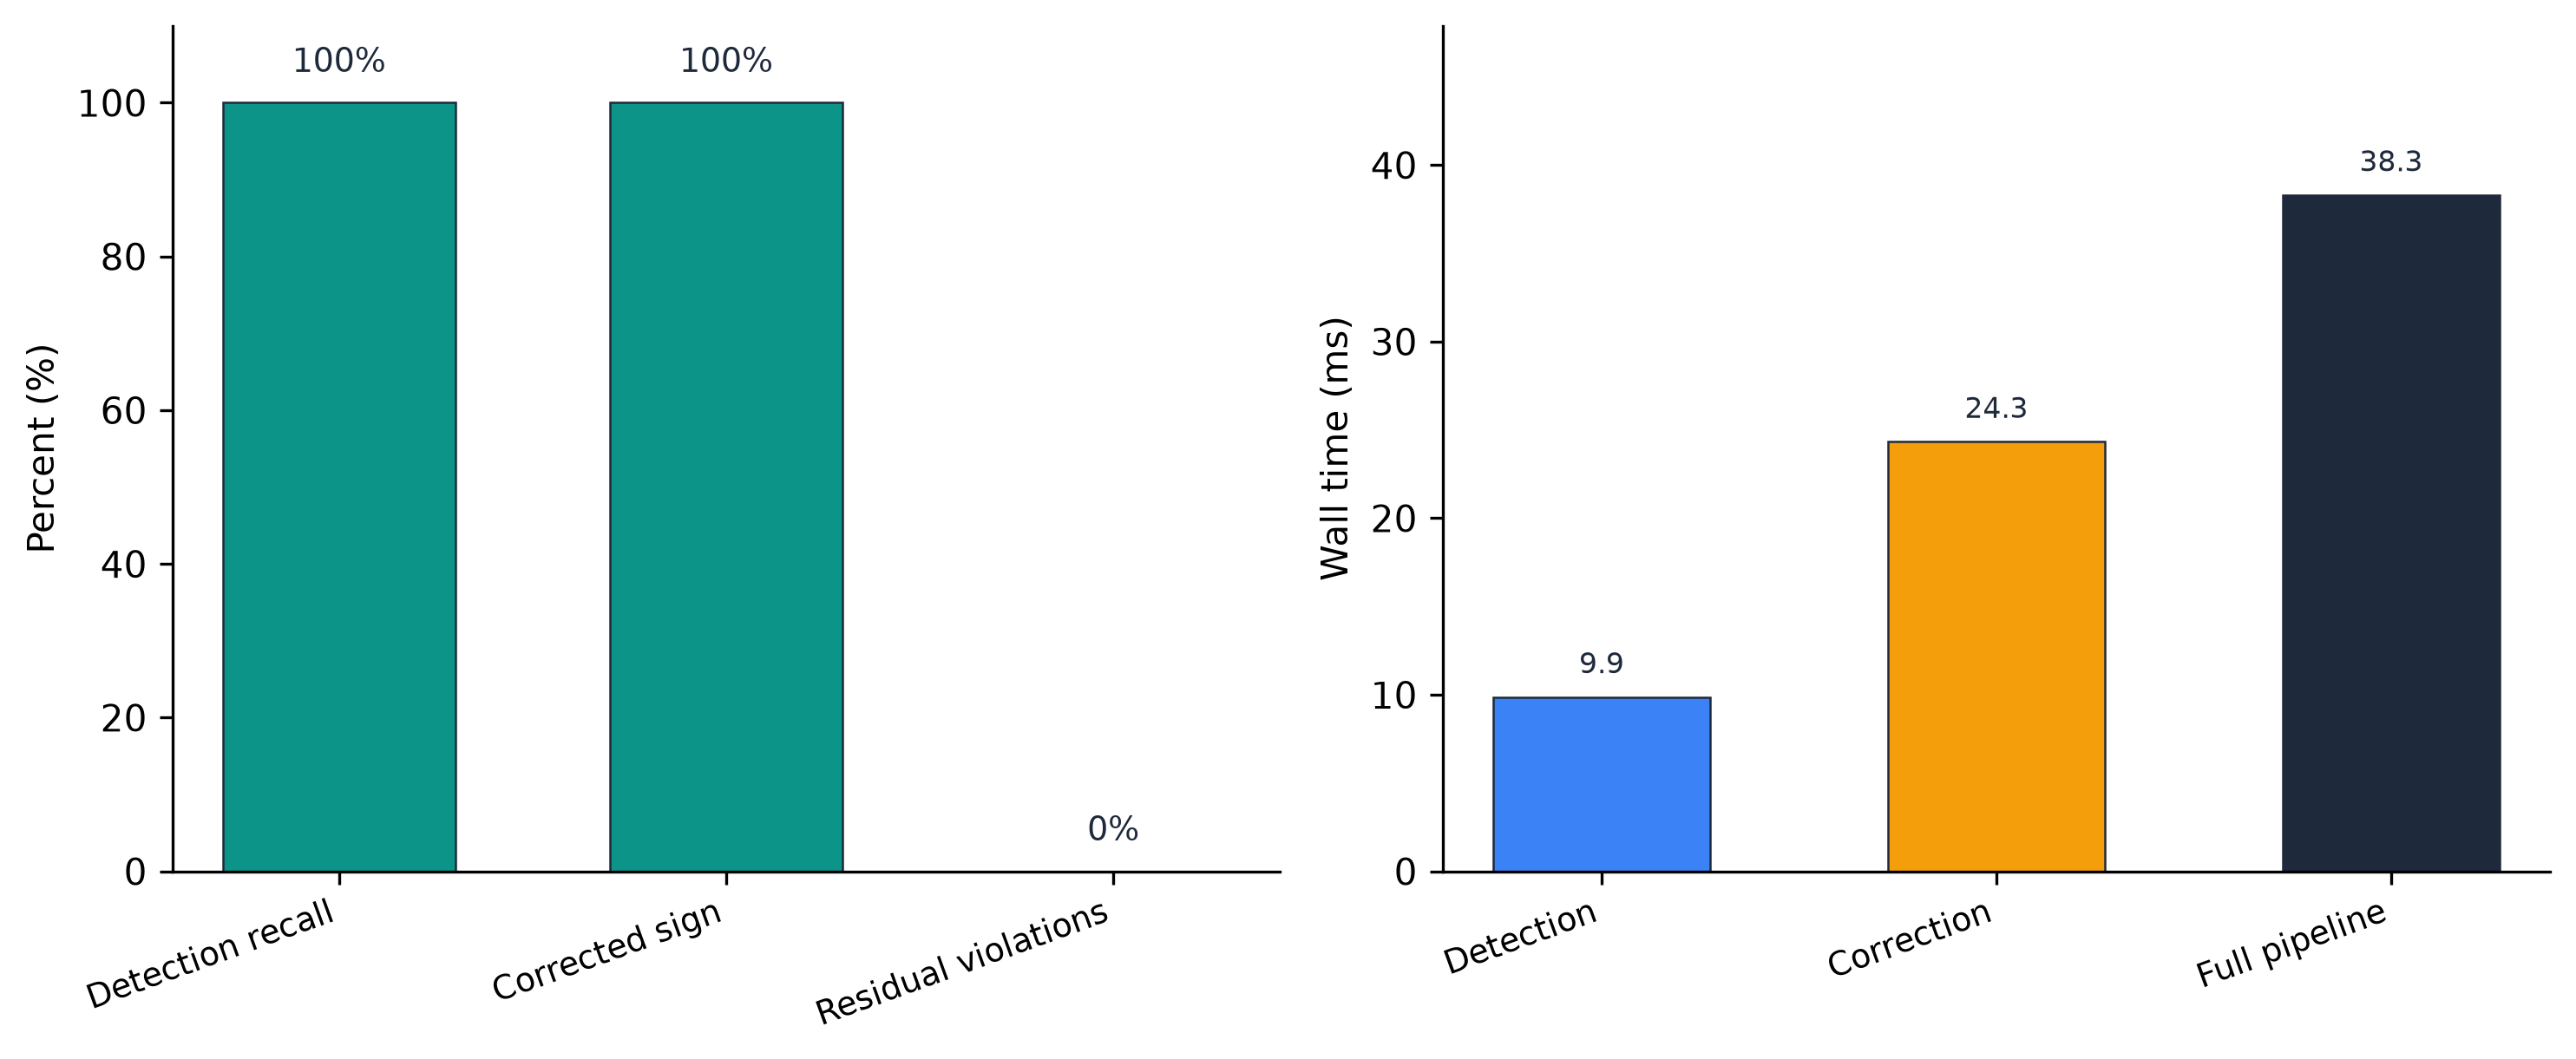
\includegraphics[width=0.95\textwidth]{fig7_af3_resource_benchmark.png}
\caption{\textbf{Figure S4.} Synthetic AF3-mimetic correction benchmark (three Childs-system peptides). Left: detection recall, correction-to-expected-sign, and residual violation rate (\%). Right: wall times (ms) for detection, correction, and the full \texttt{correct\_af3\_output} pipeline (38.3~ms total). Supports correction as a fast stereochemistry post-process, not AF3 re-inference.}
\end{figure}

\begin{figure}[h]
\centering
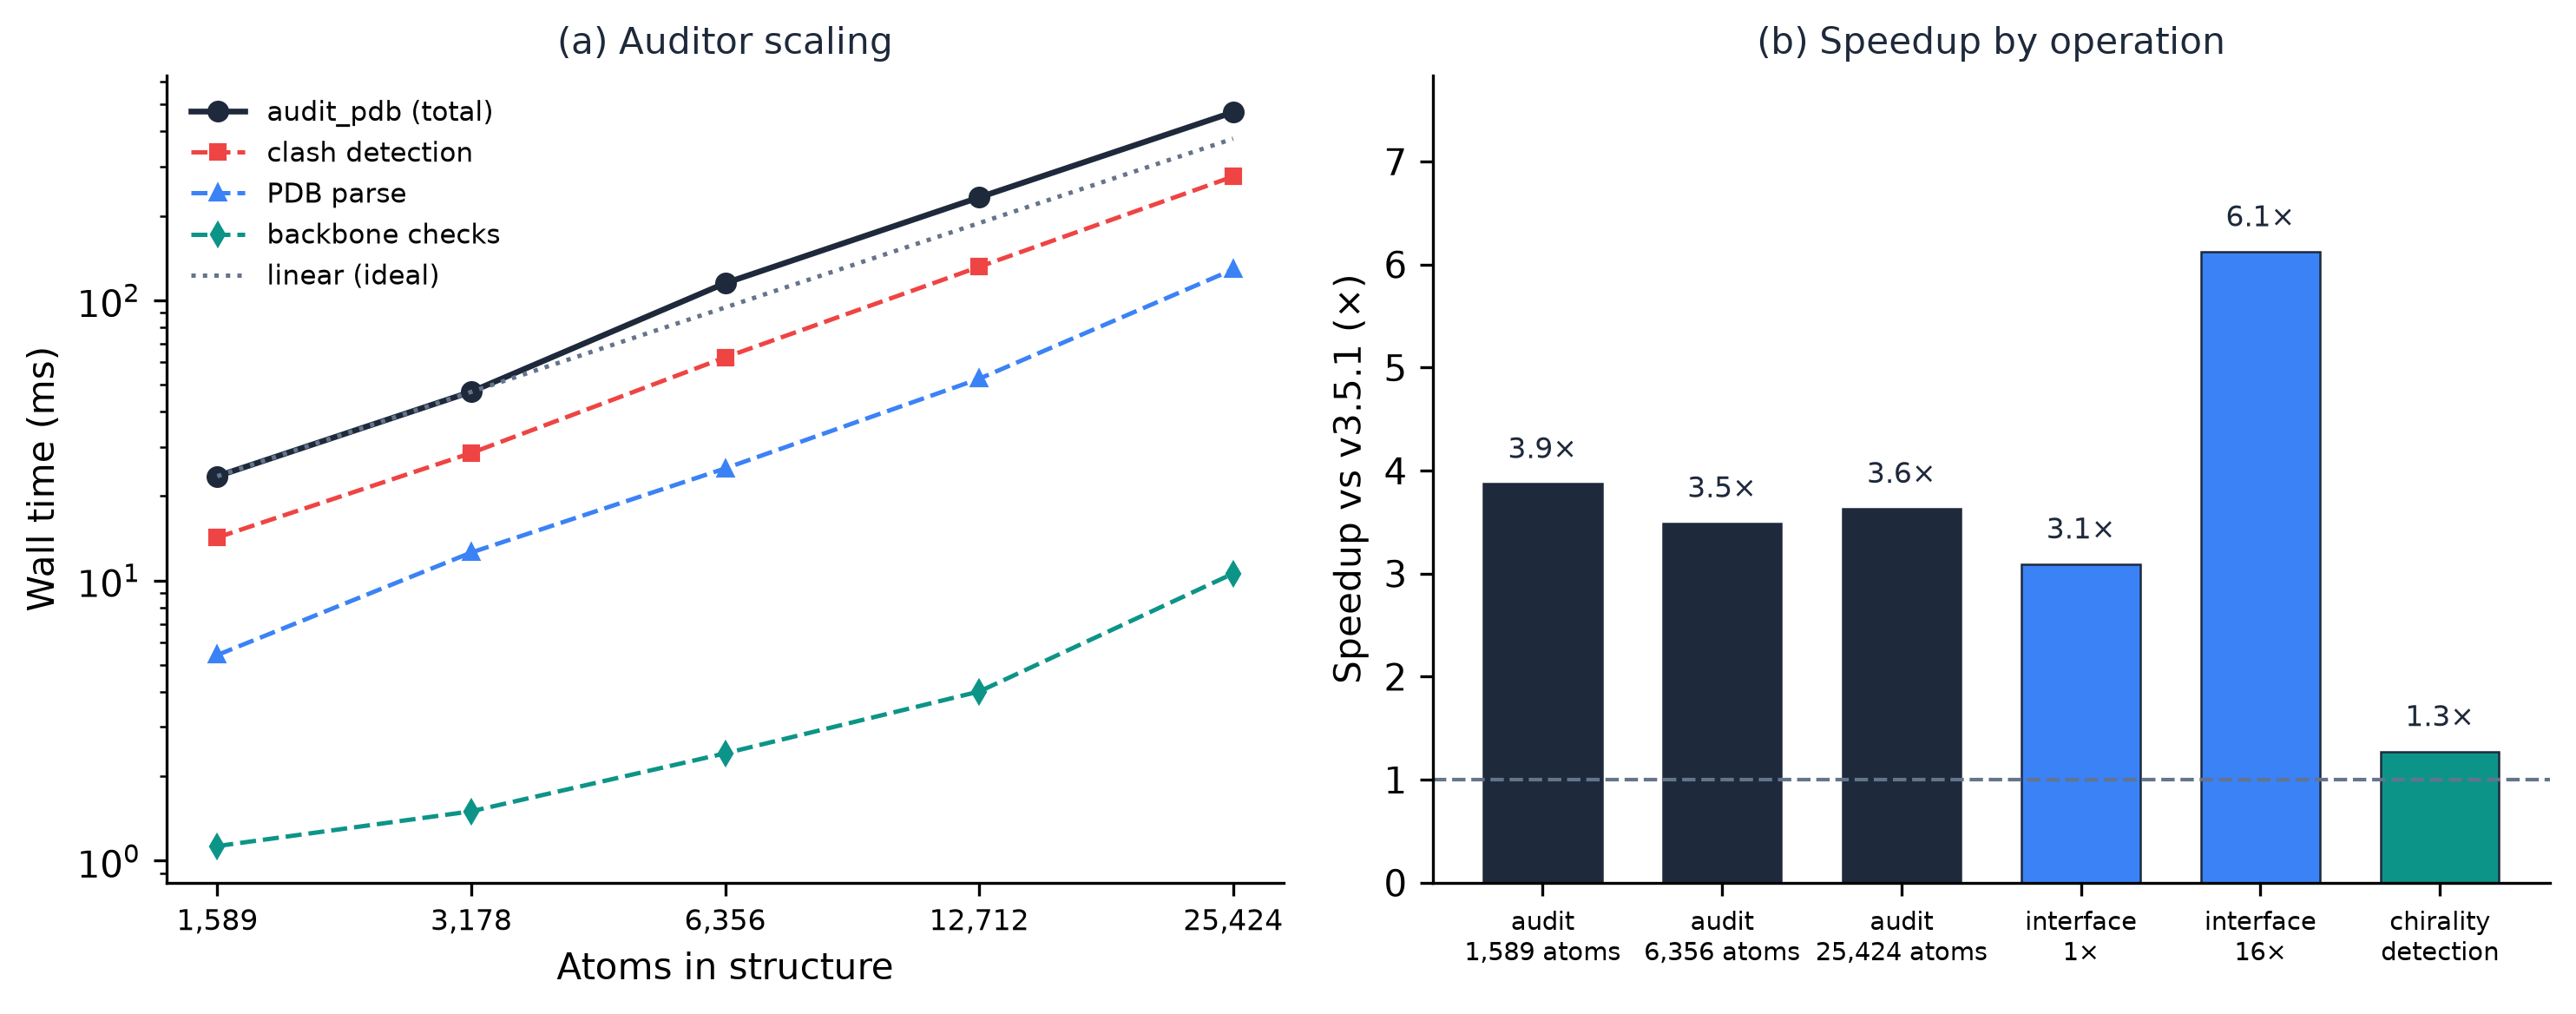
\includegraphics[width=0.95\textwidth]{fig8_performance.png}
\caption{\textbf{Figure S5.} Implementation performance. (a)~\repopath{audit_pdb} wall time versus structure size on a tiled-3IWY series (log--log), with the per-check breakdown and an ideal-linear guide; total cost is linear in atom count at 15--18~$\mu$s per atom. (b)~Speedup over v3.5.1 by operation. Medians of 7 timed repetitions after warm-up. See Supplementary Methods~\ref{sec:si_performance}.}
\end{figure}

\section{Extended statistics}
Ramachandran $n=362$ (post-5M2K exclusion): \repopath{results/ramachandran_279struct_chainfix_summary.json} --- Spearman $\rho=0.52$; Pearson $r=0.85$ (0.33 if 5M2K retained). Pilot $n=31$ Bland--Altman and bootstrap CIs: \repopath{paper/stats_extended.json} via \repopath{paper/stats_analysis.py} (seed 42). Deposition-year logistic OR$=1.60$/year; CCD clustering $\chi^2=113.78$ ($p=2.33\times10^{-16}$).

\section*{Acknowledgments (formal proofs)}
Formal verification was assisted by Aristotle (Harmonic). Lean sources and this Notes~S1 narrative are part of the ChiralFold v3.6.0 release.

\end{document}
